\appendix 
\chapter{}
\addcontentsline{toc}{chapter}{Anhang} 
\section{Vergleich der Simulationsergebnisse}
Es werden die Ergebnisse der Simulationen aus C++ und Matlab gegenübergestellt. In \ref{fig:bahn} ist klar zu erkennen, dass kein Bahnregler vorhanden ist. In beiden Simulationen folgt das Flugzeug den Querbeschleunigungen. Im Weiteren werden die Zustandsgrößen der Längs- und Seitenbewegung dargestellt.\\
\label{sec:simerg}
 \begin{minipage}{0.49\linewidth} 	
	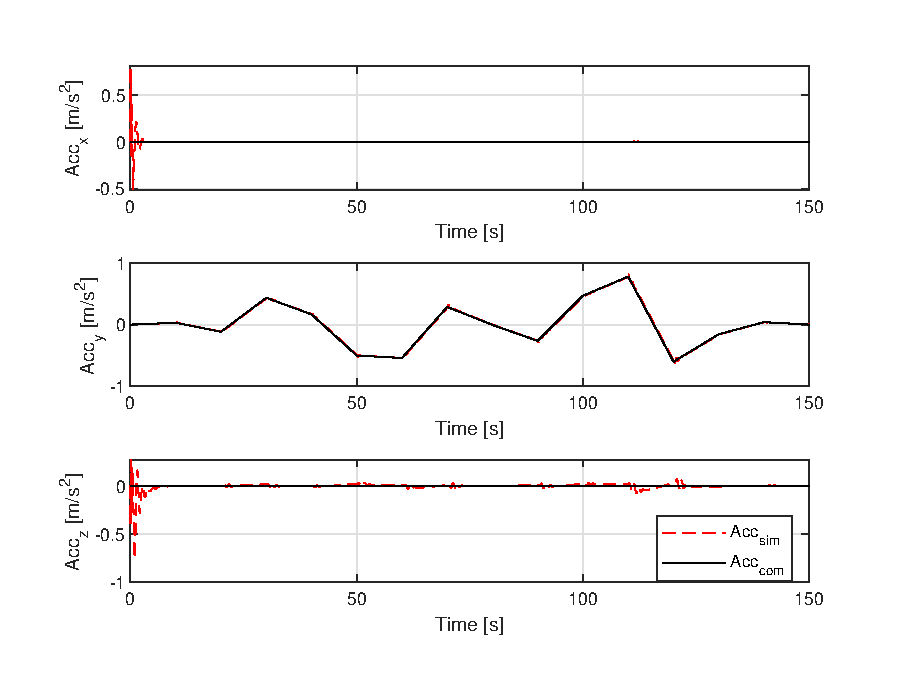
\includegraphics[width=1.0\linewidth]{querbeschleunigungen}
\end{minipage}
\begin{minipage}{0.01\linewidth}
	\hfill
\end{minipage}
\begin{minipage}{0.49\linewidth}
	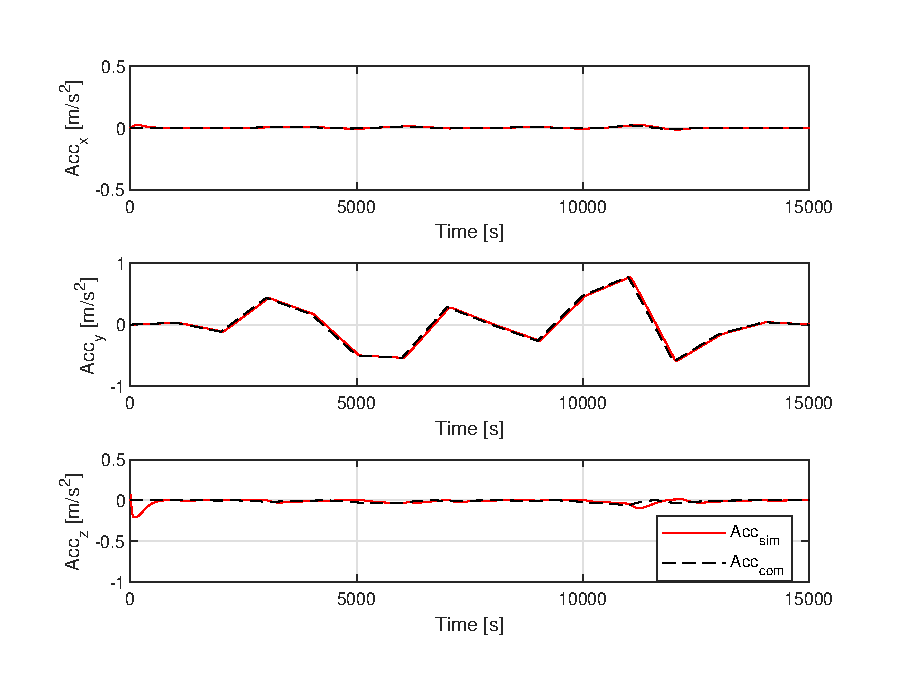
\includegraphics[width=1.0\linewidth]{matSim}
\end{minipage}
\captionof{figure}{Vergleich Querbeschleunigungen, links C++, rechts Matlab}\noindent\\
%
%
 \begin{minipage}{0.49\linewidth} 	
	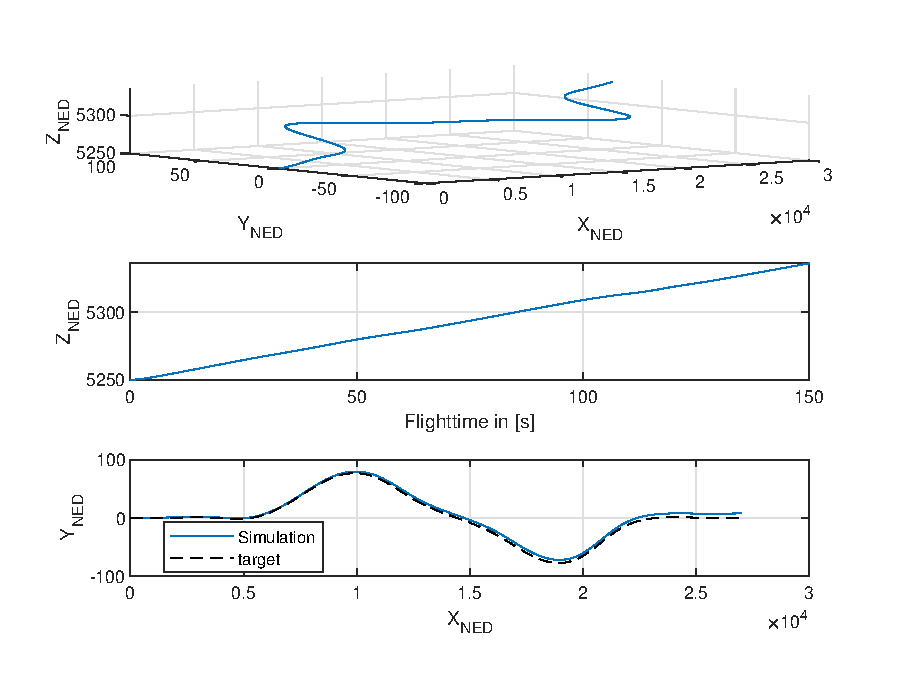
\includegraphics[width=1.0\linewidth]{trajectory}
\end{minipage}
\begin{minipage}{0.01\linewidth}
	\hfill
\end{minipage}
\begin{minipage}{0.49\linewidth}
	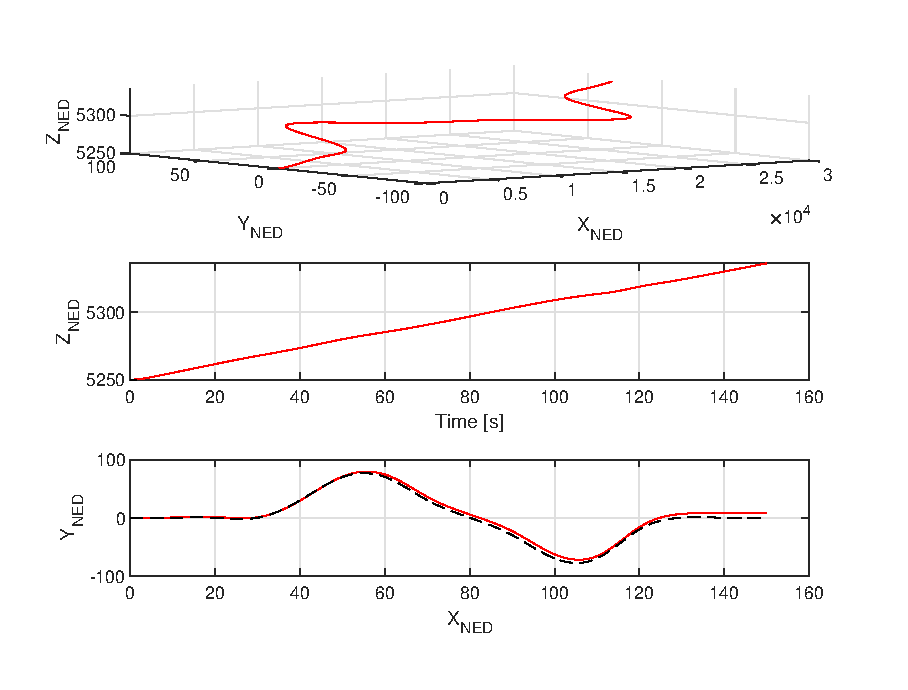
\includegraphics[width=1.0\linewidth]{trajectory_mat}
\end{minipage}
\captionof{figure}{Vergleich der Trajektorien, links C++, rechts Matlab}
\label{fig:bahn}\noindent\\
%
%
 \begin{minipage}{0.49\linewidth} 	
	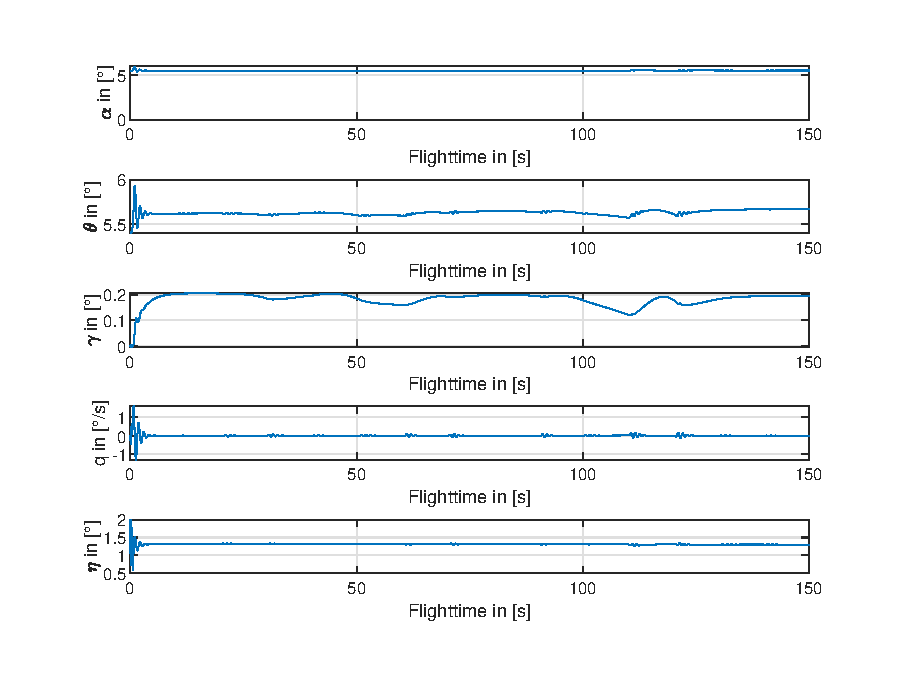
\includegraphics[width=1.0\linewidth]{pitch}
\end{minipage}
\begin{minipage}{0.01\linewidth}
	\hfill
\end{minipage}
\begin{minipage}{0.49\linewidth}
	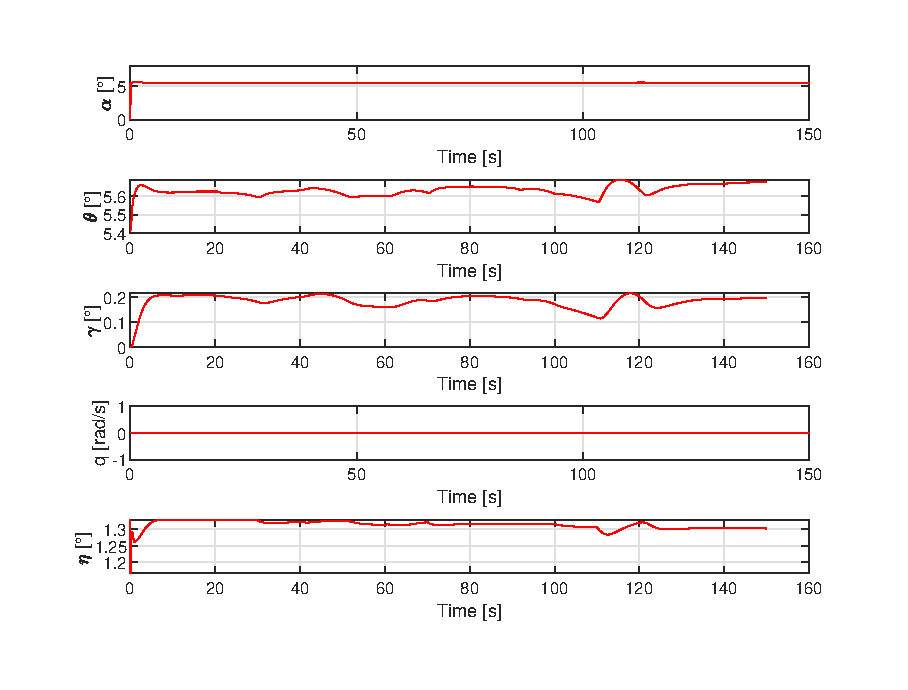
\includegraphics[width=1.0\linewidth]{pitch_mat}
\end{minipage}
\captionof{figure}{Vergleich der Längsbewegung, links C++, rechts Matlab}\noindent\\
%
%
\begin{minipage}{0.49\linewidth} 	
	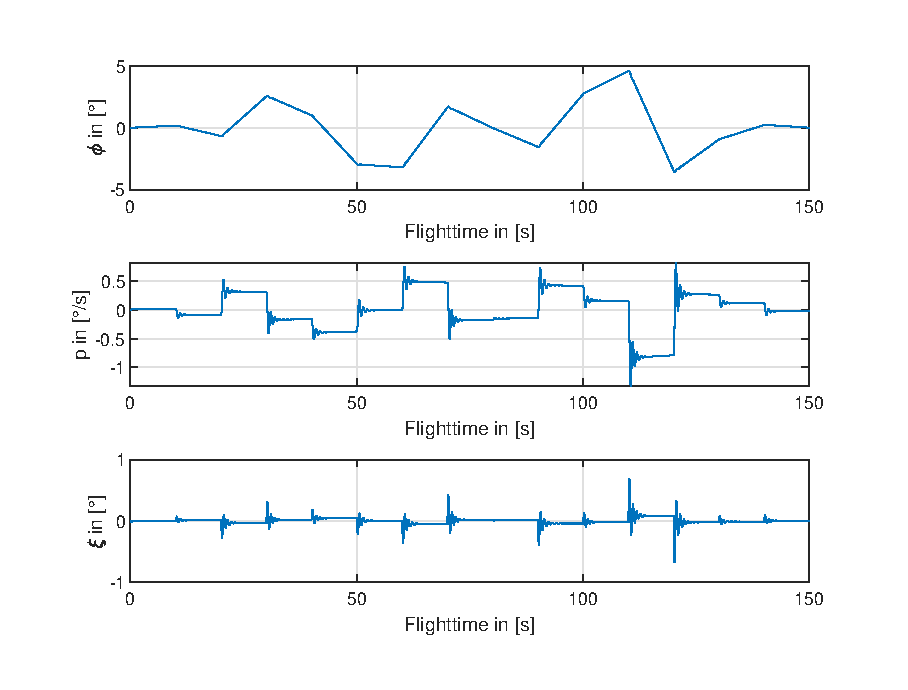
\includegraphics[width=1.0\linewidth]{roll}
\end{minipage}
\begin{minipage}{0.01\linewidth}
	\hfill
\end{minipage}
\begin{minipage}{0.49\linewidth}
	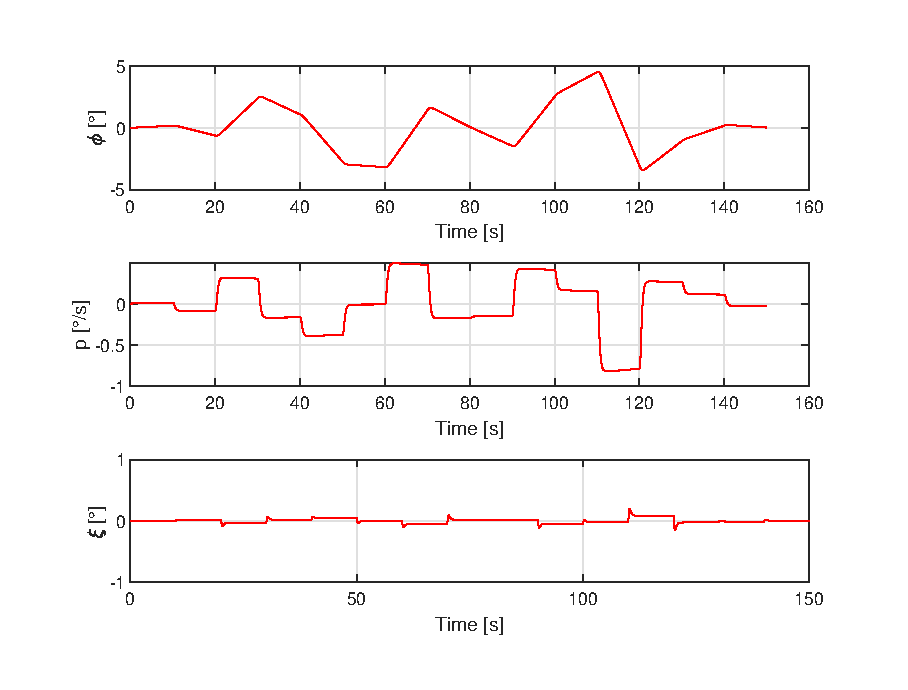
\includegraphics[width=1.0\linewidth]{roll_mat}
\end{minipage}
\captionof{figure}{Vergleich der Seitenbewegung (Rollen), links C++, rechts Matlab}\noindent\\
%
%
\begin{minipage}{0.49\linewidth} 	
	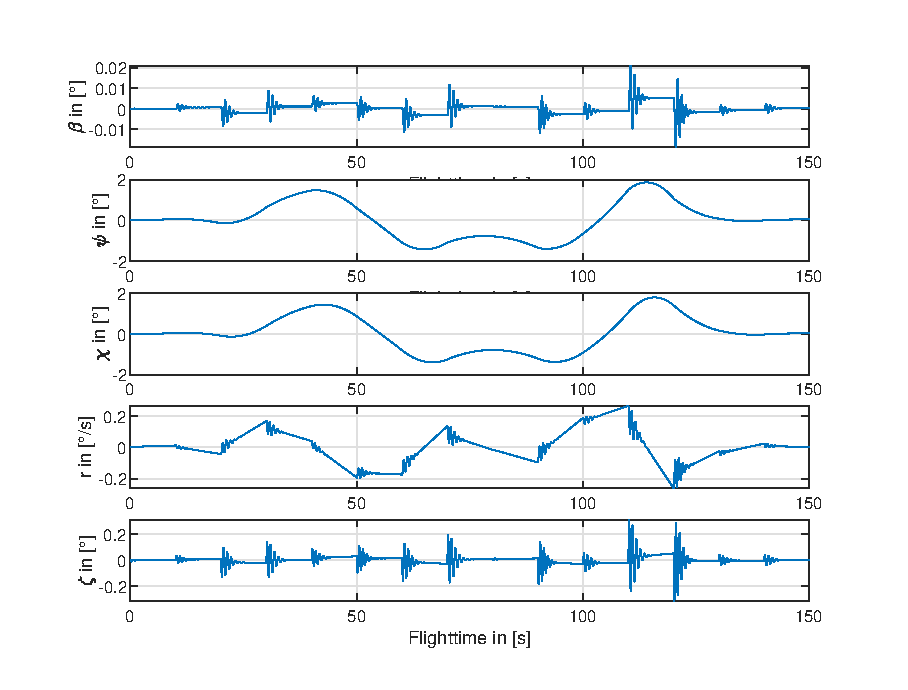
\includegraphics[width=1.0\linewidth]{yaw}
\end{minipage}
\begin{minipage}{0.01\linewidth}
	\hfill
\end{minipage}
\begin{minipage}{0.49\linewidth}
	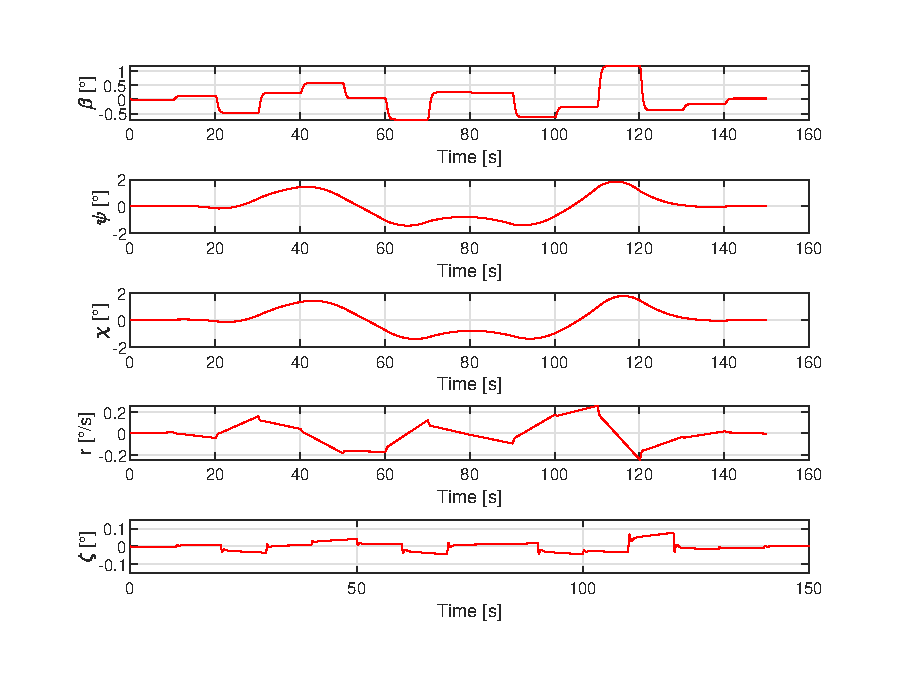
\includegraphics[width=1.0\linewidth]{yaw_mat}
\end{minipage}
\captionof{figure}{Vergleich der Seitenbewegung (Gieren), links C++, rechts Matlab}\noindent\\
%
%
\begin{minipage}{0.49\linewidth} 	
	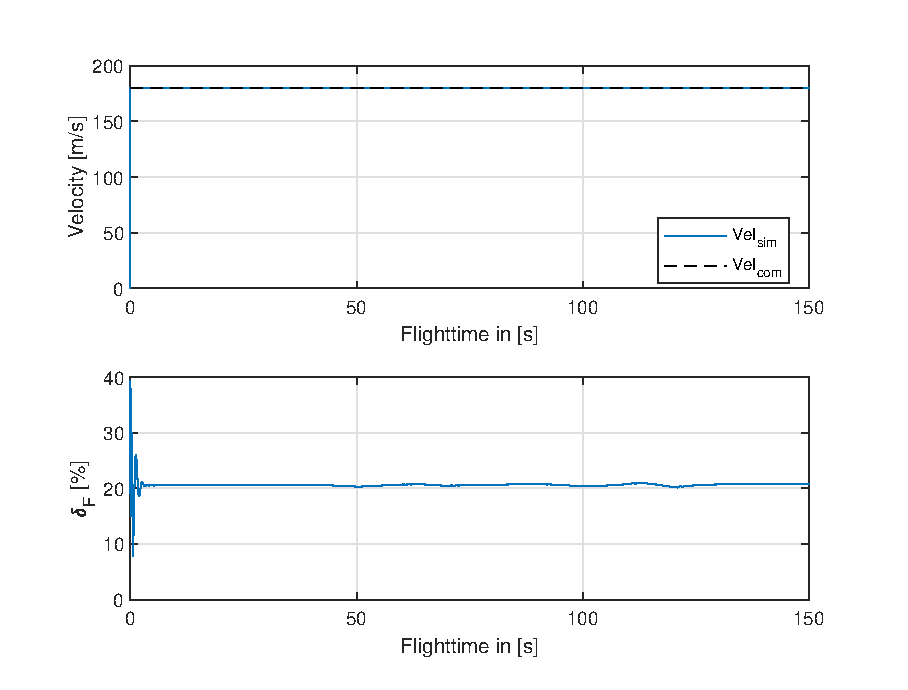
\includegraphics[width=1.0\linewidth]{vel}
\end{minipage}
\begin{minipage}{0.01\linewidth}
	\hfill
\end{minipage}
\begin{minipage}{0.49\linewidth}
	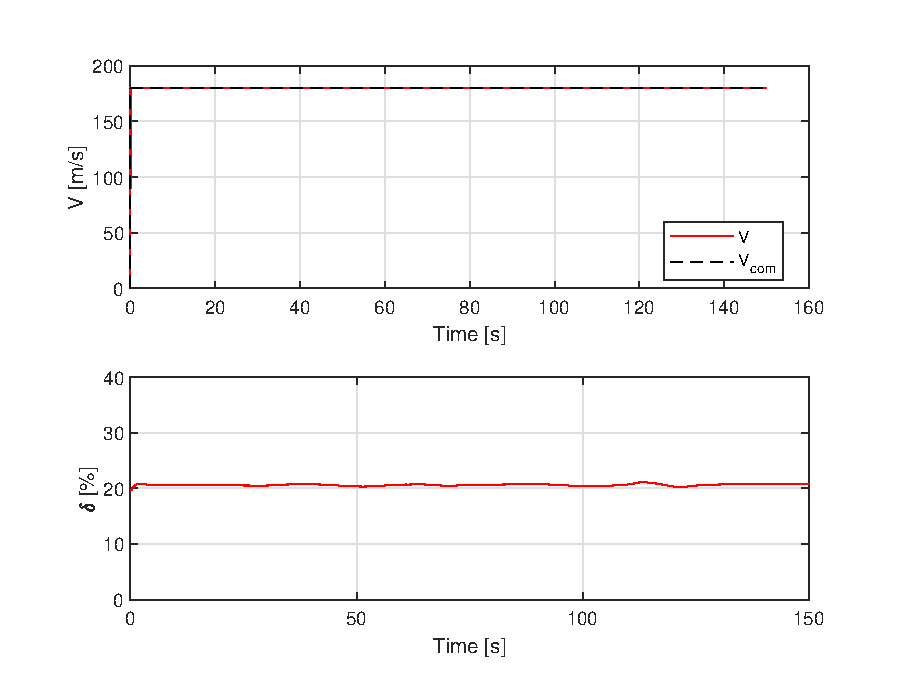
\includegraphics[width=1.0\linewidth]{vel_mat}
\end{minipage}
\captionof{figure}{Vergleich der Geschwindigkeit, links C++, rechts Matlab}\noindent\\

\section{Übersicht Dokumente}
Neben diesem Abschlussbericht, der das Vorgehen und den Aufbau der Simulation erläutern soll, sind im Ordner Documents noch weitere Dokumente hinterlegt. Diese sollen dem Nutzer bei der Bedienung unterstützen.\\
\dirtree{%
	.1 Documents.
	.2 User Manuel.
	.2 Algorithm Description Document.
	.2 Abschlussbericht.
}
